\documentclass{article}
\usepackage{graphicx} % Required for inserting images
\usepackage{listings}

\title{maze design}
\author{WO1 Clayton E. Williams}
\date{September 2023}

\begin{document}

\maketitle

\section{Project Structure}
\noindent Project structure breakdown:
\begin{lstlisting}[language=bash]
.
/data
  invalid_bfs.txt
  invalid_graph.txt
  invalid_map.txt
  map_vis.txt
  valid_map2.txt
  valid_map.txt
/doc
  design.tex
  writeup.pdf
  writeup.tex
/include
  io_helper.h
  llist.h
  matrix.h
  p_queue.h
Makefile
README.md
/src
  driver.c
  io_helper.c
  llist.c
  matrix.c
  p_queue.c
/test
  test_all.c
  test_io_helper.c
  test_matrix.c
\end{lstlisting}
\noindent data - various .txt maps for testing the project.\\
\noindent doc - documentation for the project, design plan, writeup, man page, and test plan.\\
\noindent include - custom header files for C source code files.\\
\noindent src - C source code files for project.\\
\noindent test - C source code files for unit testing.\\

\section{Data Structures Needed}
\noindent This project will rely on five main data structures. Three structs to hold the matrix, information about it, and its member variables, and a linked list with stack-like behavior and priority queue for implementing Dijkstra's Algorithm. The three structs are:
\begin{lstlisting}[language=C]
typedef struct vertex_t {
	struct vertex_t *parent;
	struct edge_t *neighbors;
	int value;
	int weight;
	char letter;
	int level;
	int num_children;
} vertex_t;

typedef struct edge_t {
	vertex_t *destination;
	struct edge_t *next;
} edge_t;

typedef struct graph_t {
	vertex_t **matrix;
	vertex_t *start;
	vertex_t *end;
	uint16_t rows;
	uint16_t cols;
	uint16_t size;
} graph_t;
\end{lstlisting}

\section{Functions Needed}
\noindent The basic functions needed are:
\begin{lstlisting}[language=C]
/*
 Callocs space for graph_t and returns pointer to the struct.
 */
graph_t *graph_create(void);

/*
 free() memory allocated for graph and its members
 */
void matrix_destroy(graph_t * graph);

/*
 Iterates over the maze file and calculates number of rows and max number of columns, setting graph.rows and graph.cols.
 */
int get_set_graph_size(FILE * fp, graph_t * graph);

/*
 Iterates over the maze file, and initializes and sets the values in the matrix based on location in the maze file. Sets vertex values, as well as confirms and denies presence of one and only one start and end point.
 */
int matrix_graph_create(FILE * fp, graph_t * graph);

/*
 Iterates over the graph, enriching each vertex with neighbors.
 */
int matrix_enrich(graph_t * graph);

/*
 Prints un-modified graph if map invalid, or no route exists.
 */
void print_graph(graph_t * graph);

/*
 Conducts a BFS against a valid map.
 */
int bfs(graph_t * graph);

/*
 If all map validation conditions are met, prints the original map, with route replaced by '.'.
 */
void print_solved(graph_t * graph);
\end{lstlisting}

\section{Project Flow}
\begin{figure}
    \centering
    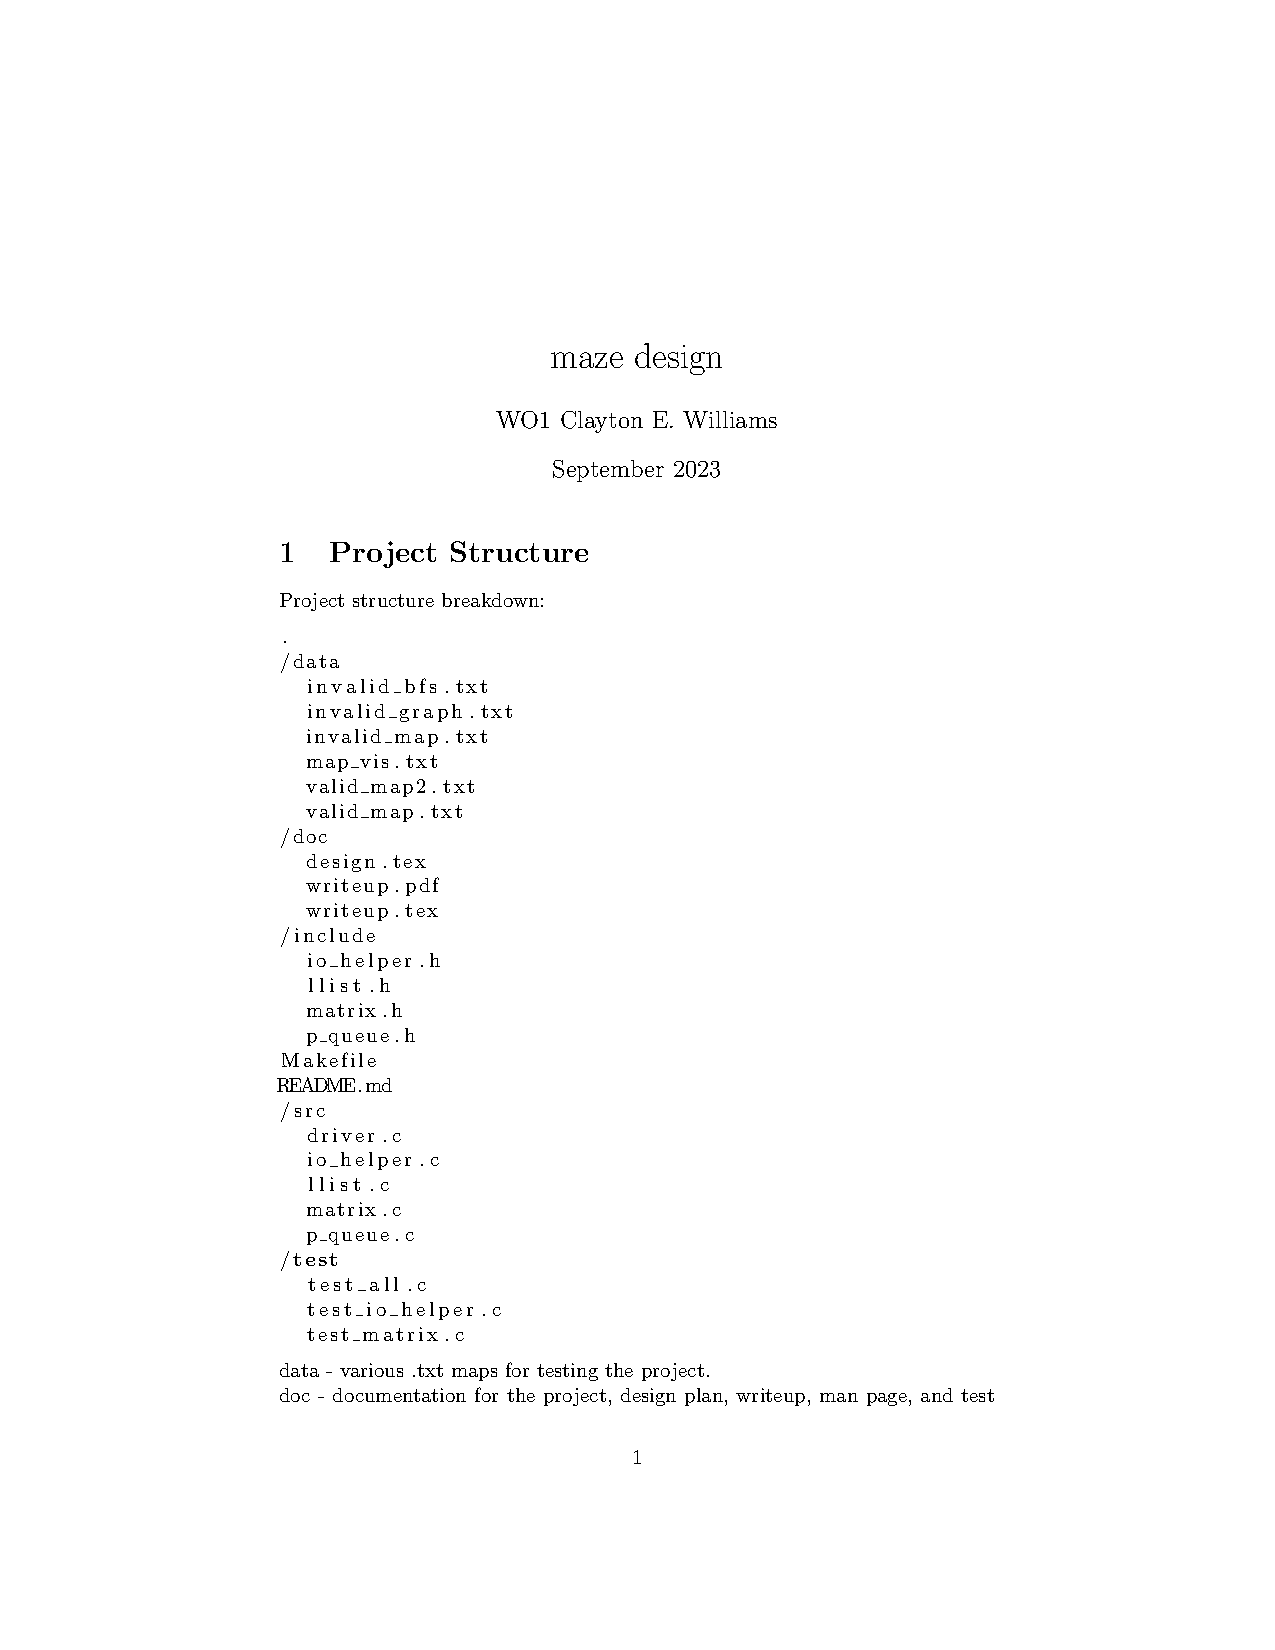
\includegraphics[width=0.5\linewidth]{design.png}
    \caption{Enter Caption}
    \label{fig:enter-label}
\end{figure}
\end{document}

